%%%%%%%%%%%%%%%%%%%%%%%%%%%%%%%%%%%%%%%%
%---------- Segundo Capitulo ----------
\chapter{Fundamenta\c{c}\~ao Te\'orica}
\label{chap:desenv}
%%%%%%%%%%%%%%%%%%%%%%%%%%%%%%%%%%%%%%%%

Com o objetivo de simular o efeito coro, al�m do \textit{SpeechEasy} que integra \textit{hardware} e \textit{software} num dispositivo eletr\^onico personalizado, oferecendo op\c{c}\~oes de tamanho, e diferenciais como adapta\c{c}\~ao instant\^anea e menor efeito de oclus\~ao \cite{Microson2015}. Existem algumas ferramentas que trabalham somente com \textit{software} e que exercem essa fun\c{c}\~ao juntamente com algum dispositivo de reprodu\c{c}\~ao de a\'udio que contenha microfone. 
\begin{figure}[H]
	\centering
	%\begin{measuredfigure}
	\caption{Op\c{c}\~oes de tamanho do SpeechEasy. \label{fig:gdimotes}}
	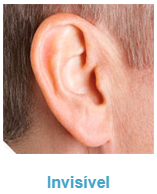
\includegraphics[height=5cm]{./figuras/speecheasy_invisivel_figure.png} \quad
	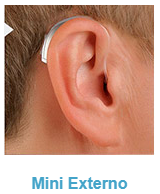
\includegraphics[height=5cm]{./figuras/speecheasy_pequeno_figure.png} \quad
	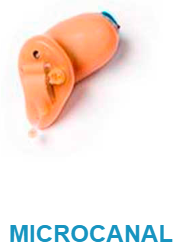
\includegraphics[height=5cm]{./figuras/speecheasy_microcanal_figure.png} \newline
	\fonte{\cite{Microson2015}}
	%\end{measuredfigure}
\end{figure}

Para computadores de mesa e notebooks com sistema operacional Windows, existe o "\textit{Software} Mais Flu\^encia Win DAF/FAF \textit{Software}", desenvolvido em 2009 pelo Henrique Confessor, \'e \textit{freeware} podendo ser distribu\'ido e utilizado livremente, disponibilizado gratuitamente para \textit{download} no site da "Abra Gagueira" \cite{Confessor2009}. Sua interface simples, permite somente duas configura\c{c}\~oes, atraso e frequ\^encia, apresenta apenas dois bot\~oes auxiliares que tem as fun\c{c}\~oes de fechar e exibir uma tela com as informa\c{c}\~oes sobre o \textit{software}, como: vers\~ao, e-mail para contato e o link para o blog do autor. \'E o \textit{Software} mais funcional relatado neste documento, atende somente a funcionalidade de simular o efeito coro, n\~ao traz nenhum diferencial. 

\begin{figure}[H]
	\centering
	%\captionsetup{width=0.97\textwidth}
	\caption[Interface do software Mais Flu\^encia Win DAF/FAF]{Interface do software Mais Flu\^encia Win DAF/FAF. \label{fig:figuramaisfluencia}}
	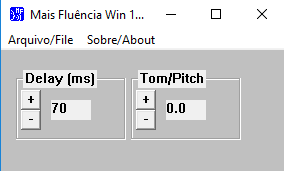
\includegraphics[height=7cm]{./Figuras/maisfluencia_figure.png}% <- formatos PNG, JPG e PDF
	\fonte{O Autor.}
\end{figure}

Para dispositivos m\'oveis com sistema operacional Android ou IOS existe o \textit{DAF Assistant} que tem uma vers\~ao gratuita, por\'em com limite de tempo para sua utiliza\c{c}\~ao, j\'a sua vers\~ao paga que n\~ao possui essa restri\c{c}\~ao, custa aproximadamente 13 reais na \textit{Play Store} e 33 reais no \textit{Itunes}, variando de acordo com pre�o do dollar \cite{Artefact2012}. 

O \textit{DAF Assistant} possui uma interface intuitiva, contendo as op\c{c}\~oes de configurar atraso e frequ\^encia, traz apenas dois bot\~oes repons\'aveis por iniciar ou parar a reprodu\c{c}\~ao do efeito coro. Existem op\c{c}\~oes que n\~ao est\~ao vis\'iveis na tela, ficando acess\'iveis somente quando pressionado o bot\~ao de configura\c{c}\~ao do celular (dependendo de cada dispositivo), exibindo a op\c{c}\~ao de fechar o aplicativo, ou ir para uma tela de preferencias, onde \'e poss\'ivel ativar a utiliza\c{c}\~ao de um \textit{headset bluetooth}, al\'em do \textit{auto mute}, \textit{mute after} e configurar a sensibilidade da fala em baixa, normal ou alta. 
\begin{figure}[H]
	\centering
	%\captionsetup{width=0.97\textwidth}
	\caption[Interface do aplicativo DAF Assistant]{Interface do aplicativo DAF Assistant. \label{fig:figuradafassistant}}
	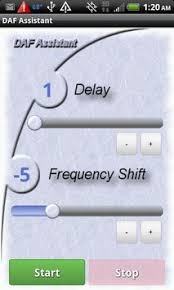
\includegraphics[height=10cm]{./Figuras/dafassistant_figure.jpg}% <- formatos PNG, JPG e PDF
	\fonte{\cite{Artefact2012}}
\end{figure}

Com o intuito de fornecer o \sigla{FAA}{\textit{feedback} auditivo atrasado}, tamb\'em para a plataforma Android existe o aplicativo "Terapia para a gagueira - FAA", que \'e gratuito e traz informa\c{c}\~oes interessantes sobre o tratamento da gagueira, como dicas de como utilizar o aplicativo e informa��es adicionais sobre tratamentos que melhoram a flu\^encia da fala. Lembrando que diferente da \sigla{RAA}{retroalimenta\c{c}\~ao auditiva atrasada}, o FAA trabalha apenas com o atraso na reprodu\c{c}\~ao da voz, n\~ao alterando a frequ\^encia com que a voz \'e reproduzida \cite{Age2017}.

A interface do aplicativo Terapia para a gagueira - FAA cont\'em muita informa\c{c}\~ao, possuindo muitos bot\~oes, isso se da pelo fato de oferecer diversas funcionalidades al\'em do FAA, como: oferece um espelho utilizando a c\^amera frontal do dispositivo, op\c{c}\~ao de gravar o \'audio enquanto faz a utiliza\c{c}\~ao do aplicativo, disponibiliza um metr\^onomo para controle do r\'itimo da fala e um v\'ideo contendo informa\c{c}\~oes sobre o tratamento da gagueira. Apesar de gratuito comt\'em muitas propagandas, oque pode ocasionar inc\^omodo em alguns usu\'arios. 

\begin{figure}[H]
	\centering
	%\captionsetup{width=0.97\textwidth}
	\caption[Interface do aplicativo Terapia para a gagueira - FAA]{Interface do aplicativo Terapia para a gagueira - FAA. \label{fig:figuraterapiaparagagueira}}
	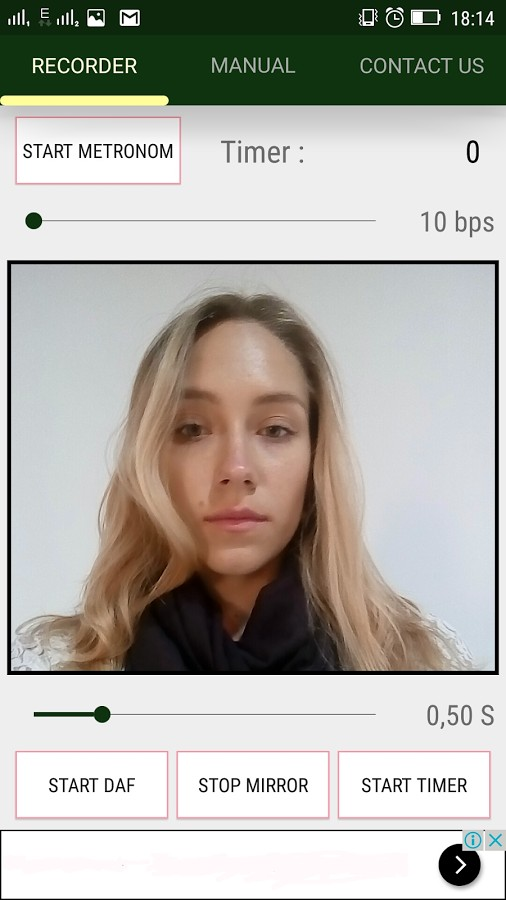
\includegraphics[height=10cm]{./Figuras/terapiaparagagueira_figure.jpg}% <- formatos PNG, JPG e PDF
	\fonte{\cite{Age2017}}
\end{figure}







